%%body for test 1


%%formulation 

\ques{21}  You are tasked with advising the Prince George's County School Board (PGCSB) on the locations of two new magnet schools they intend to open. These two schools will serve 7 different townships. Let $h_i$ be the number of students from township $i$ that have qualified for the magnet program: 


	\begin{center}
$\begin{array}{| l || l | l| l| l| l|l|l|} \hline \text{Township, $i$} & 1 & 2 & 3 & 4 & 5 & 6 & 7 \\ \hline
\text{Number of Students, $h_i$} & 100 & 60 & 80 & 120 & 60 & 150 & 20 \\ \hline \end{array}	$
	\end{center}

The figure below will be used to help make the decision, where each of the $n=7$ nodes $I = \{1,2,...,7\}$ correspond to the townships and the nodes $J=\{4, 6, 7\}$ in dashed boxes are the possible locations for the schools. The weight on each edge $(i,j)$ corresponds to direct distances (in km) between $i$ and $j$.  Let the distance $d_{ij}$ be the length of the shortest path in this graph between nodes $i$ and $j$.  

\begin{figure}[h!t]
\begin{center}
  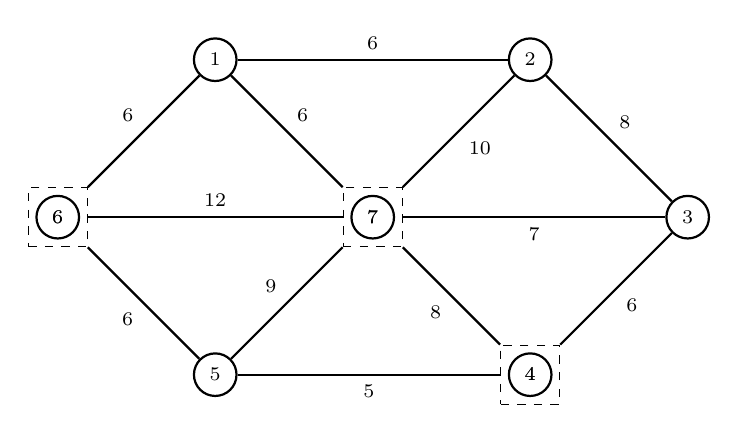
\begin{tikzpicture}
    [font=\scriptsize,
    %    node/.style={shape=circle,draw=blue!60,fill=blue!20,minimum width=0.5cm,thick},
    node/.style={shape=circle,draw=black,minimum width=0.5cm,thick},
    node1/.style={shape=rectangle,draw=black,minimum width=0.75cm,minimum height=0.75cm,dashed},
    arc/.style={->,>=stealth,thick},
    edge/.style={thick}]

    \node (1) [node] at (-2,2) {1};
    \node (2) [node] at (2,2) {2}; 
    \node (3) [node] at (4,0) {3};
   % \node (3) [node1] at (-1,0.75){};      
    \node (4) [node] at (2,-2) {4};
   % \node (5) [node1] at (4,2){};     
    \node (5) [node] at (-2,-2) {5};
    \node (6) [node] at (-4,0) {6};
   % \node (6) [node1] at (-2,-0.5){};      
    \node (7) [node] at (0,0) {7};
  %  \node (7) [node1] at (2,-1){};     
  %  \node (8) [node1] at (4,0){};    
    \node (4) [node1] at (2,-2) {4};
    \node (6) [node1] at (-4,0) {6};
    \node (7) [node1] at (0,0) {7};
          
    \draw [edge] (1) to node [auto] {6} (2);
    \draw [edge] (2) to node [auto] {8} (3);
    \draw [edge] (3) to node [auto] {6} (4);
    \draw [edge] (4) to node [auto] {5} (5);
    \draw [edge] (5) to node [auto] {6} (6);
    \draw [edge] (6) to node [auto] {6} (1);
    \draw [edge] (1) to node [auto] {6} (7);
    \draw [edge] (2) to node [auto] {10} (7);
    \draw [edge] (3) to node [auto] {7} (7);
    \draw [edge] (4) to node [auto] {8} (7);
    \draw [edge] (5) to node [auto] {9} (7);
    \draw [edge] (6) to node [auto] {12} (7);
     
          

  \end{tikzpicture}
\end{center}
\end{figure}

The possible schools at nodes 4, 6 and 7 can serve up to 350, 350 and 450 students, respectively. All of the students from a township are required to attend the same magnet school. The PGCSB wants to minimize the total distance traveled to school by all students, opening only two schools. 

\vspace{0.3 cm}

\noindent
In what follows, use the decision variables
\[
X_j = \binvar{if a school is opened at node $j$},  j \in J,
\]
and 
\[
Y_{ij} = \binvar{if township $i$'s students go to school in township $j$}, i \in I,~ j \in J.
\]

\newpage

\begin{parts}
    \pts{3} Write an objective function that minimizes the total distance traveled by all students.  

\vfill
    
    \pts{4} Write the constraint that ensures that the number of students attending the school at location 4 is not more than the capacity of that school. 

\vfill
    
    \pts{3} Write the constraint ensuring that exactly two schools are opened. 

    \vfill

    \pts{3} Write the constraint that ensures that the students from township 2 are served by some school. 

    \vfill
    
    \pts{3} Write a constraint or a list of constraints that ensure that no students are sent to school at location 4 if the school at location 4 is not opened. 
    
    \vfill
    
   \newpage
    
    \pts{3}  The townspeople at location 6 are in an uproar. The current model could potentially send their kids to a school in a different township, even if a magnet school is opened in their town. Write a constraint that guarantees that the students in township 6 are sent to school in township 6 if a school is opened in township 6. 
    
    

\vspace{3in}

\pts{2} After solving the model and making your recommendations, the PGCSB returns to ask you whether building a single school with enough capacity to house the students in all townships will decrease the total distance traveled by all students. One board member indicates that the distance {\bf must} increase since using fewer schools puts some students farther from a magnet school. Another board member notes that using smaller schools forces some students to travel further due to capacity constraints. Which argument is correct? Or are both wrong? Mark the claim that is correct: 

\begin{itemize}
\item[$\square$] Using a single school forces the total distance to go up. 

\item[$\square$] Using a single school with unlimited capacity forces the total distance to go down. 

\item[$\square$] Using a single school with unlimited capacity may change the total distance traveled but without looking closely at the given data you can't determine which direction the total distance traveled will change. 
\end{itemize}

\vspace{0.33in}

\end{parts}

\newpage

\ques{24} The Brothers that ran the NEHI Bottling Company have retired and sold their business. In the decades since the bottling industry has changed and customers no longer return bottles to the store for deposit. Instead customers recylce at home. Local townships provide recycling pick ups and transport the recycling to temporary storage. Trucks operated by a regional recycling center must pick up the recycling from each town's storage and bring it to the center. Assume that the regional recycling center has 3 trucks that can carry 8 tons of recycling each. The NEHI brothers have taken over the operation of the recycling center and want to find routes for the trucks to minimize the total distance traveled in collecting all of the recycling. The drivers always start and end their deliveries at the center, designated as node 0.  The center serves 10 towns and the recycling load $h_i$ for each township $i$ is given below. 


\begin{center}
\begin{tabular}{|l||c|c|c|c|c|c|c|c|c|c|} \hline
Township, $i$ 
&  1	&	2	&	3	&	4	&     5	&	6	&	7	&	8	&   9    &     10
\\
\hline
Tons of recylcing, $h_i$ 
&   2	&	3	&	2	&	1	&	1	&	3	&	1	&	3	&    2   &   2 \\\hline
\end{tabular}
\end{center}

You have determined that the distances between the center and the towns are given by a symmetric matrix.  An entry in this matrix $d_{ij}$ 
gives the distance between location $i$ and location $j$, where $i$ and $j$ range from $0$ to $10$.

You copied down part of the model for the Vehicle Routing problem from a copy of the course text:
\[
\begin{array}{llllr}
  \min & \Sum_{(i,j) \in \cE} d_{ij} X_{ij} & \\
\mbox{s.t.} & \Sum_{j \in \cV | i < j} X_{ij} + \Sum_{j \in \cV |j<i} X_{ji} & = ? & i =
1,\ldots,10 & (\rm{a}) \\
&  \Sum_{j=1}^{10} X_{0j}  = 2m & & & (\rm{b}) \\
& X_{ij} \in \{0,1\} & & \forall (i,j) \in \cE. &
\end{array}
\]
You have figured out that the graph should be $\cG = (\cV,\cE)$ where $\cV
= \{0,1,\ldots,10\}$ and $\cE = \{ (i,j) | i < j, i,j \in \cV\}$.  

\vspace{0.5cm}

\begin{parts}
  \pts{2} Unfortunately, you spilled coffee on your text during a late night study session and can't make out the right-hand side of constraint (a). What number should replace the question mark? 

\newpage

  \pts{6} You use an integer programming solver to find a solution to the formulation as described. The solver provides the following solution: $X_{0,1}=X_{0,2}=X_{0,3}=X_{0,4}=X_{0,5}=X_{0,6}=X_{1,2}=X_{3,4}=X_{5,6}=X_{7,8}=X_{8,9}=X_{9,10}=X_{7,10}=1$.  All other $X_{ij} = 0$.  Draw the vehicle routes that this solution describes.

\vspace{3in}

 

  \pts{5} Is the solution provided by the solver in part (b) a valid solution to the problem faced by the recycling center? Why or why not?

  \vspace{2in}
  
  \pts{2} Suppose the solver returns the routes 0-1-5-3-0, 0-4-2-8-9-0, and 0-6-10-7-0. Find the weight of the load that the truck visiting towns 2, 4, 8 and 9 must carry. 
  

  
  
  \newpage
  \pts{6} One of the NEHI brothers claims that adding the cycle elimination constraint $X_{04} + X_{24} + X_{28} + X_{89} + X_{09} \leq 4$ will get rid of the solution mentioned in part (d). His brother agrees but thinks that a constraint of the form   
\[
\sum_{i,j \in S, i<j} X_{ij} \le \abs{S} - \ell (S)
\]
would be better. He argues that here $S = \{2,4,8,9\}$ and $\abs{S} = 4$. {\bf Find $\ell(S)$ and write down the associated constraint explicitly (i.e. it starts out $X_{2,4}+\cdots$).}\vspace{1.5in}

\pts{3} Find a path involving the center and towns 2, 4, 8 and 9 that would not be allowed by your answer to (e) but would be allowed by the cycle elimination constraint. 
\vspace{2in}

\end{parts}
\ques{4} Mark each statement as true or false. \\

\smallskip
\begin{parts}
\pt \underline{\hspace{1cm}} There is no way to run external (non-Excel) programs from VBA. \vspace{0.33in}

\pt \underline{\hspace{1cm}} The symbol ``+'' is used to tie together strings to build a longer string in VBA; e.g., if \texttt{name} is a string variable:  \verb!"Name:  " + name!


\end{parts}

\newpage

\ques{16}
Consider the following graph:
\begin{center}
  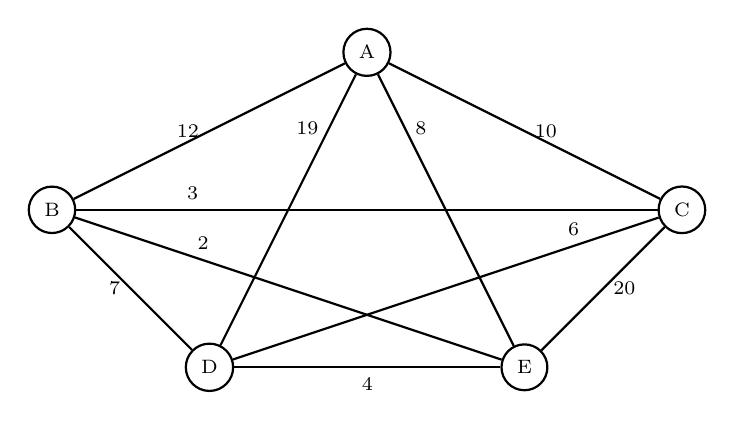
\begin{tikzpicture}
    [font=\scriptsize,
    %    node/.style={shape=circle,draw=blue!60,fill=blue!20,minimum width=0.5cm,thick},
    node/.style={shape=circle,draw=black,minimum width=0.5cm,thick},
    arc/.style={->,>=stealth,thick},
    edge/.style={thick}]
          
    \node (A) [node] at (0,3) {A};
    \node (B) [node] at (-4,1) {B};
    \node (C) [node] at (4,1) {C};
    \node (D) [node] at (-2,-1) {D};
    \node (E) [node] at (2,-1) {E};

    \draw [edge] (A) -- (B) node[pos=0.5,left] {$12$};
    \draw [edge] (A) -- (C) node[pos=0.5,right] {$10$};      
    \draw [edge] (A) -- (D) node[pos=0.2,left] {$19$};
    \draw [edge] (A) -- (E) node[pos=0.2,right] {$8$};              
    \draw [edge] (B) -- (C) node[pos=0.2,above] {$3$};
    \draw [edge] (B) -- (D) node[pos=0.5,left] {$7$};
    \draw [edge] (B) -- (E) node[pos=0.3,above] {$2$};
    \draw [edge] (C) -- (D) node[pos=0.2,above] {$6$};
    \draw [edge] (C) -- (E) node[pos=0.5,right] {$20$};     
    \draw [edge] (D) -- (E) node[pos=0.5,below] {$4$};

  \end{tikzpicture}
\end{center}
The numbers adjacent to the edges give the costs $c_{ij}$.  You are told to run Prim's algorithm to construct a minimum cost spanning tree, starting at node $A$. 

\vspace{0.5cm}

\begin{parts}
\pts{2} Based on Prim's algorithm, which is the first edge you should add to your tree?

\vfill

\pts{2}  Based on Prim's algorithm, which is the second edge you should add to your tree?
\vfill

\pts{2}  Based on Prim's algorithm, which is the third edge you should add to your tree?

\vfill

\pts{2}  Based on Prim's algorithm, which is the fourth edge you should add to your tree?

\vfill

\pts{2} What is the TOTAL cost of the tree you get by running Prim's algorithm?

\newpage

  \pts{6} Prim's algorithm is (circle one):  
\begin{enumerate}
\item an exact algorithm
\item a heuristic algorithm
\end{enumerate} 
which uses a (circle one):
\begin{enumerate}
\item constructive approach
\item local search approach
\end{enumerate}
so it will (circle one):
\begin{enumerate}
\item find the guaranteed optimal solution to the problem no matter how long it takes
\item attempt to find a near-optimal solution quickly, with no guarantee of optimality
\end{enumerate}


 \vspace{2cm}

You may find the following pseudo-code for Prim's algorithm useful. 
\vspace{0.5cm}
	
\noindent	{\bf Given:}  $n$ cities, start city, and cost matrix {\bf c} = $(c_{ij})$ \medskip 
	
\noindent	Set $tree\_cost \leftarrow 0$ \\
    Set $T \leftarrow \emptyset$ \\
    Set $S \leftarrow \{\text{start city}\}$ \\
	$V \leftarrow \{1,\ldots,n\}\setminus S$ is the collection of unselected cities\\
	{\bf Until} $V = \emptyset$ {\bf do}\\
	\phantom{XXXXXX} Let $(i,j)$ be a least cost edge with $i \in S$ and $j \in V$ \\
	\phantom{XXXXXX} $S \leftarrow S \cup \{j\}$  \\
	\phantom{XXXXXX} $V \leftarrow V \setminus \{j\}$ \\
	\phantom{XXXXXX} {\bf If } $i < j$ {\bf Then} \\
	\phantom{XXXXXXXXX} $tree\_cost \leftarrow tree\_cost + c_{ij}$ \\
	\phantom{XXXXXXXXX} $T \leftarrow T \cup \{(i,j)\}$ \\
	\phantom{XXXXXX} {\bf Else}\\
 		\phantom{XXXXXXXXX} $tree\_cost \leftarrow tree\_cost + c_{ji}$ \\
			\phantom{XXXXXXXXX} $T \leftarrow T \cup \{(j,i)\}$ \\
    \phantom{XXXXXX} {\bf End if}\\
    {\bf End loop}
    
\noindent {\bf Return} $tree\_cost$ and tree $T$ 
	

\end{parts}


%\newpage

%%bonus question

%\bques{8} Telecommunication companies are often concerned with the design of local access and transport area (LATA) networks that provide special access service through a local exchange facility.  Suppose we have 8 possible hub locations that are to be connected to 10 customers.  The company requires that between 3 and 6 hubs be used; the additional cost associated with opening the hubs depends on their quantity and is not linear, as seen in the following table.

%\begin{center}
%\begin{tabular}{ccccc}
% & \multicolumn{4}{c}{Number of Hubs Used} \\ \hline
% &  3 	&	4	&	5	&	6	\\ \hline
%Cost (\$) & 40,000 & 60,000 & 70,000 & 75,000 \\ 
%\hline
%\end{tabular}
%\end{center}

%\noindent Using the following indices, sets, data, and decision variables write an objective function and the necessary constraints to ensure that between 3 and 6 hubs are used and the appropriate cost is paid for using that number of hubs.

%\begin{tabbing}
%\noindent{\bf Indices and Sets}\\[0.2cm]
%\hspace*{.5cm} \= $i\in I$ \hspace{2.8cm} \= customers, $I=\{1,2,...,10\}$ \\
%\> $j\in J$ \> possible hub locations, $J=\{1,2,...,8\}$\\
%\> $k\in K$ \> possible total number of hubs used, $K=\{3,4,5,6\}$\\[0.2cm]
%\noindent{\bf Data}\\[0.2cm] 
%\> $cHubs_k$ \> cost of  opening $k$ hubs\\[0.2cm]
%\noindent{\bf Decision Variables}\\
%\> $y_j$ \> 1 if node $j$ is the location of a hub, 0 otherwise\\
%\> $w_{k}$ \> 1 if $k$ hubs are used, 0 otherwise\\[0.2cm]
%\end{tabbing}